\subsection{Tab}

\subsubsection{MOSFET}
\noindent Det nye simulerede samlede tab i MOSFET'en ses på figur~\ref{fig:simulering_power_MOSFET}. Simuleringen foregår på samme måde som ved sektion ~\ref{MOSFETsimtab}, hvor gate-modstanden i stedet er ændret til de $13.7\ohm$. Her aflæses den samlede afsatte effekt i MOSFET'en til ca. $3.2\watt$. 

\begin{figure}[H]
	\center
	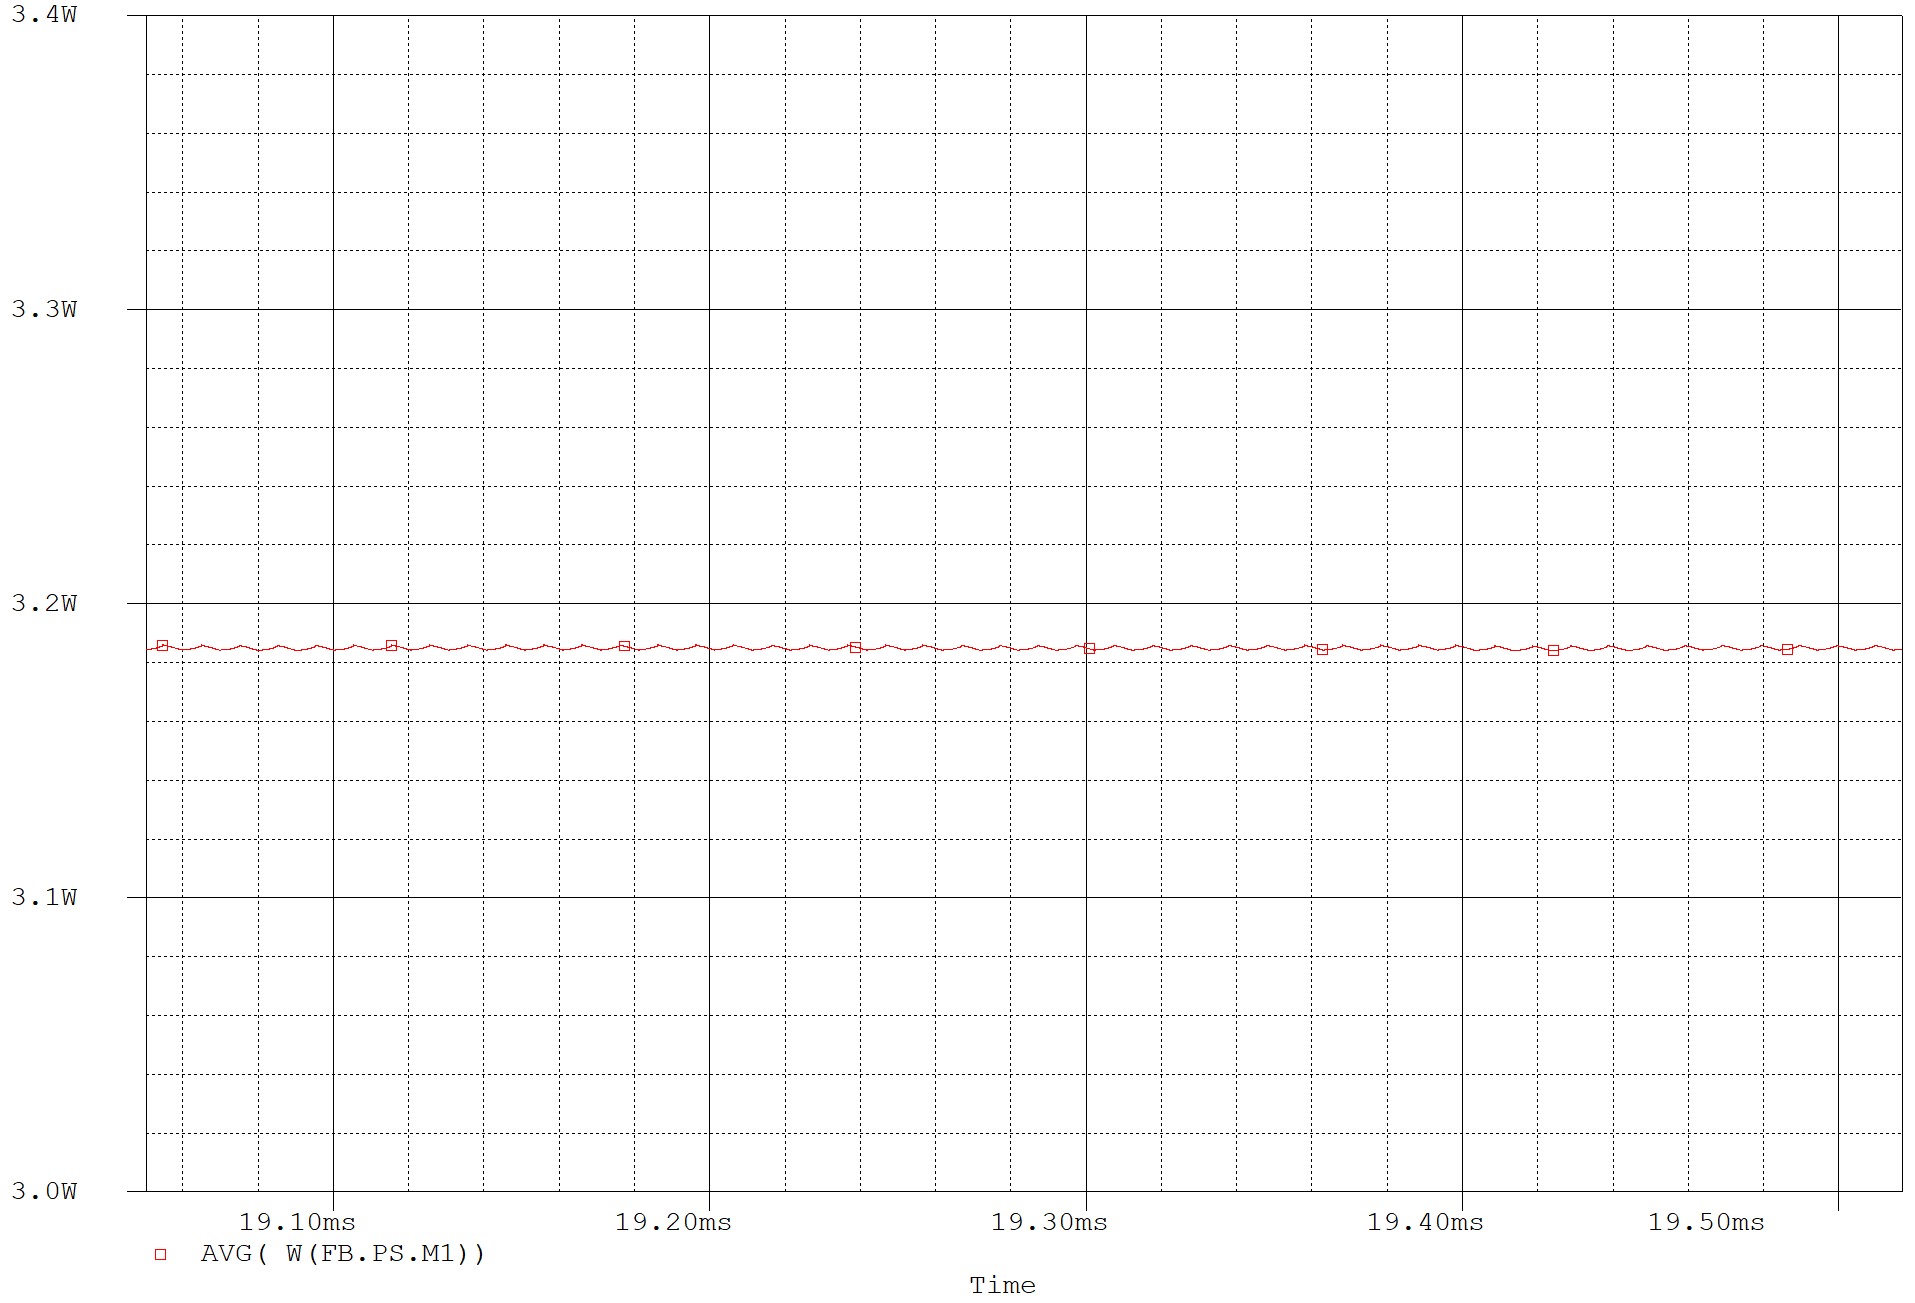
\includegraphics[max width=0.9\linewidth]{/tex/3iteration/billeder/Simulering/simulering_power_MOSFET.png}
	\caption{Simulering af effektafsættelse i MOSFET}
	\label{fig:simulering_power_MOSFET}
\end{figure}

\subsubsection{Snubber-kredsløb}
\noindent Tabet i snubber-kredsløbene simuleres ved, at kigge på tabene i snubber-modstandene, da det er her effekten bliver afsat. Figur~\ref{fig:simulering_power_snubber_MOSFET} viser effekten afsat i det primære snubber-kredsløb. Her aflæses effekten til $234m\watt$. Figur~\ref{fig:simulering_power_snubber_diode} viser effekten afsat i det sekundære snubber-kredsløb. Her aflæses effekten til $74m\watt$. 

\begin{figure}[H]
	\center
	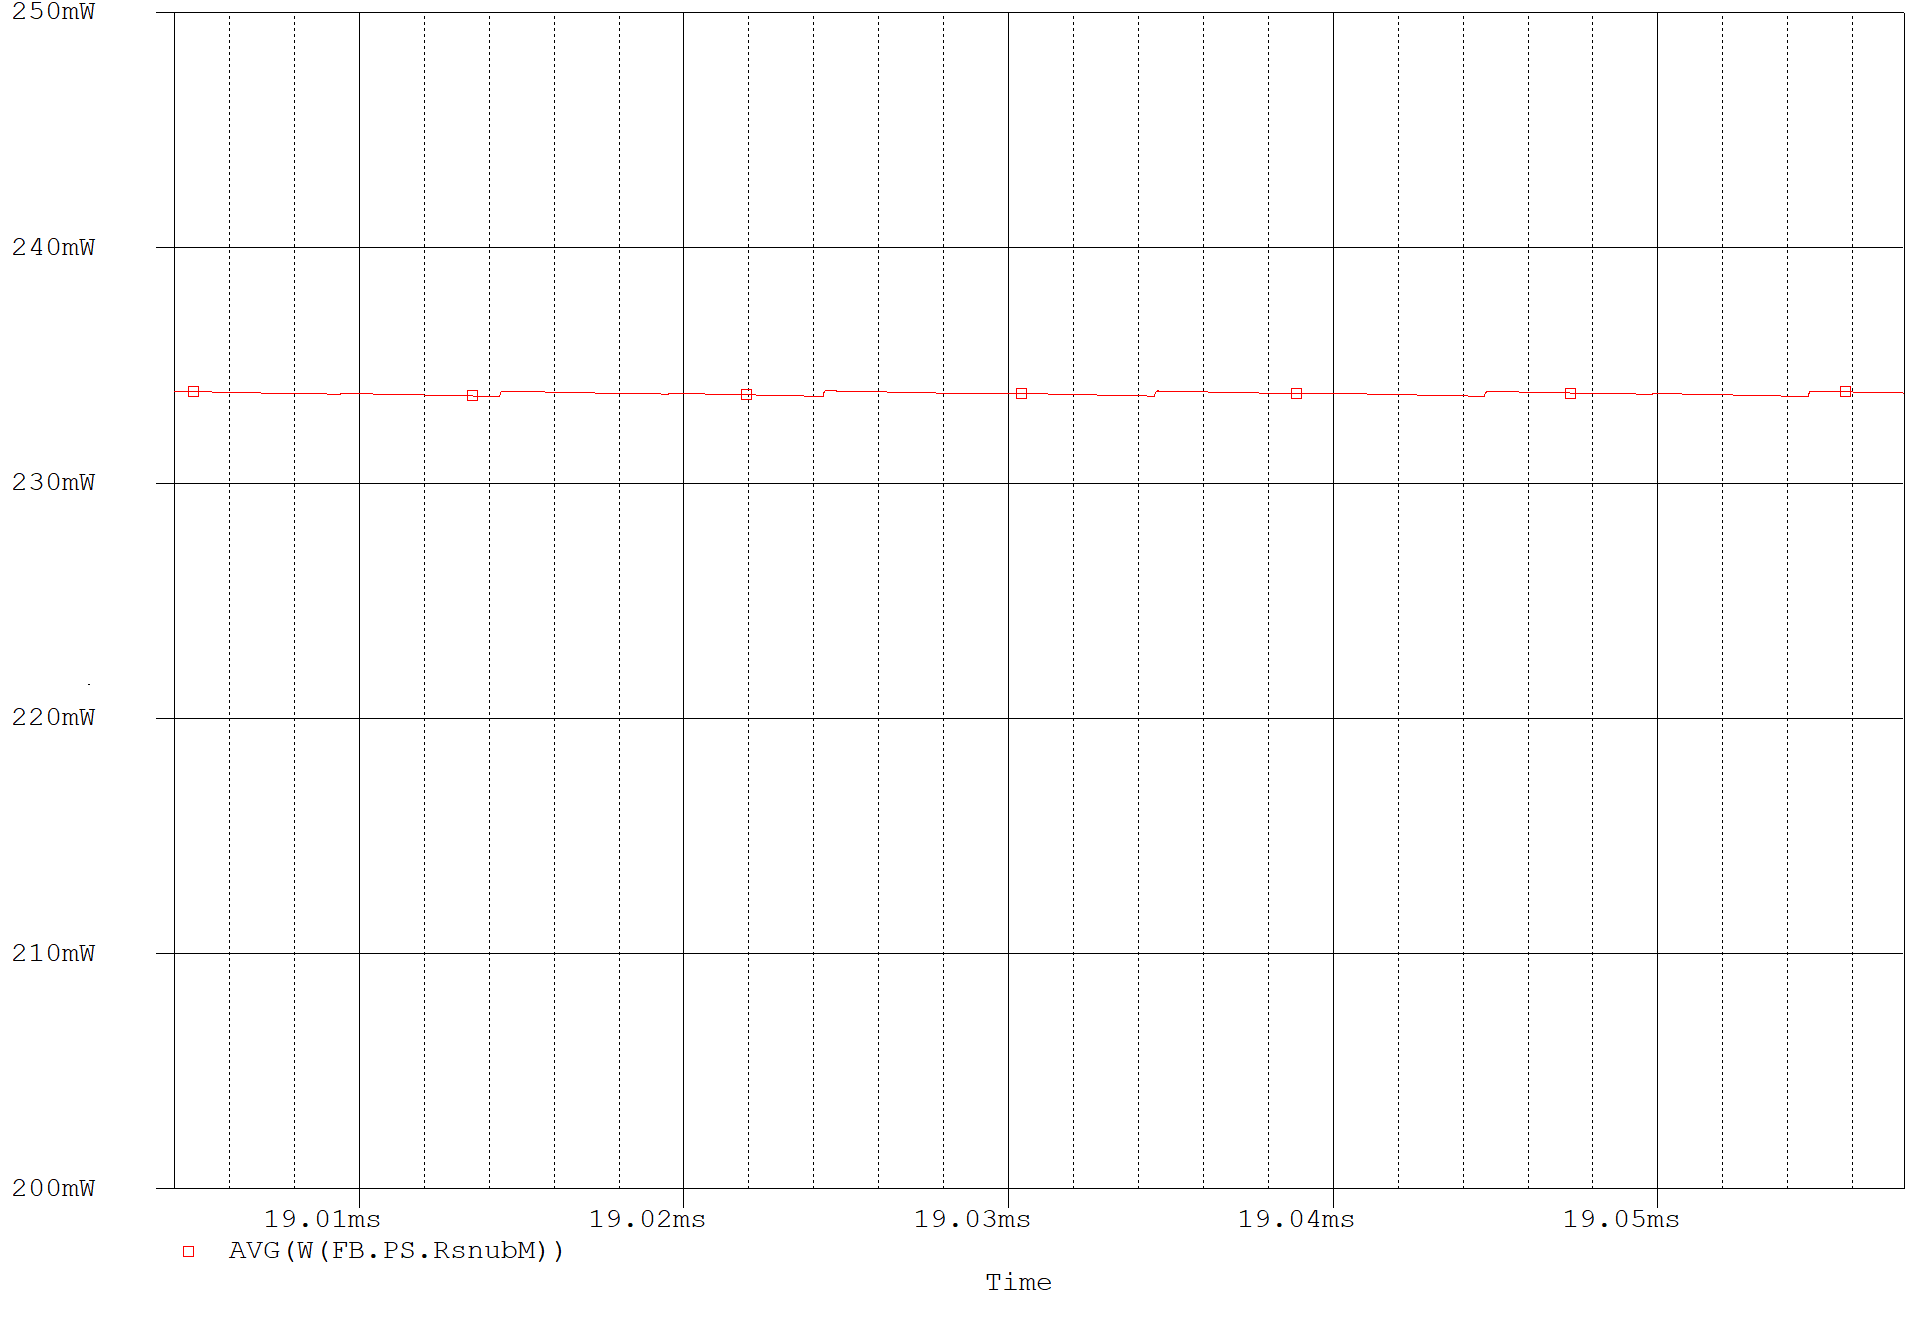
\includegraphics[max width=0.9\linewidth]{/tex/3iteration/billeder/Simulering/simulering_snubber_power_MOSFET.png}
	\caption{Simulering af effektafsættelse i det primære snubber-kredsløb}
	\label{fig:simulering_power_snubber_MOSFET}
\end{figure}

\begin{figure}[H]
	\center
	\includegraphics[max width=0.9\linewidth]{/tex/3iteration/billeder/Simulering/Simulering_snubber_power_diode.png}
	\caption{Simulering af effektafsættelse i det sekundære snubber-kredsløb}
	\label{fig:simulering_power_snubber_diode}
\end{figure}

\subsubsection{Oversigt over simuleret tab}
\begin{table}[H] 			
	\centering
	\begin{tabularx}{\textwidth}{|X|l|l|}
		\hline
		\textbf{\large Komponent} & \multicolumn{2}{|l|}{\textbf{\large Tab}} \\ \hline
		& A & S	\\ \hline
		\textbf{Transformator samlet} & $1.46\watt$ & $1.62\watt$ \\ \hline 
		Kernetab & $366m\watt$ & $311m\watt$ \\ \hline
		Kobbertab & $1.09\watt$ & $1.31\watt$ \\ \hline
		& &	\\ \hline
		\textbf{MOSFET samlet} & $2.54\watt$ & $3.2\watt$ \\ \hline
		Conduction-tab & $1.06\watt$ & 	\\ \hline
		Switch-tab & $1.48\watt$ & 		\\ \hline
		& &	\\ \hline
		\textbf{Diode} & $1.13\watt$ & $1.47\watt$ \\ \hline
		& &	\\ \hline
		\textbf{CS modstands tab} & $1.52\watt$ & $2.03\watt$ \\ \hline
		& &	\\ \hline
		\textbf{Snubber-kredsløb} & $220.9m\watt$ & $308m\watt$ \\ \hline
		Primær snubber	& $132.5m\watt$	& $234m\watt$		\\ \hline
		Sekundær snubber &	$88.4m\watt$ &	$74m\watt$		\\ \hline
		& &	\\ \hline
		\textbf{Total tab} & $6.87\watt$ & $8.63\watt$ \\ \hline
	\end{tabularx}
	\caption{Oversigt over analyseret og simuleret tab}
	\label{tab:simulering_tab_3}
\end{table}

Figur~\ref{fig:simulering_power_samlet} viser en simulering af converterens indgangseffekt(grøn) og udgangseffekt(rød). Indgangseffekten er aflæst til $61.4\watt$, og udgangseffekten er aflæst til $52.7\watt$. Differensen på dette er det samlede effekttab i converteren, som er regnet til $8.7\watt$. Det viser, der er taget højde for de dominerende tab i tabsberegningerne. 

\begin{figure}[H]
	\center
	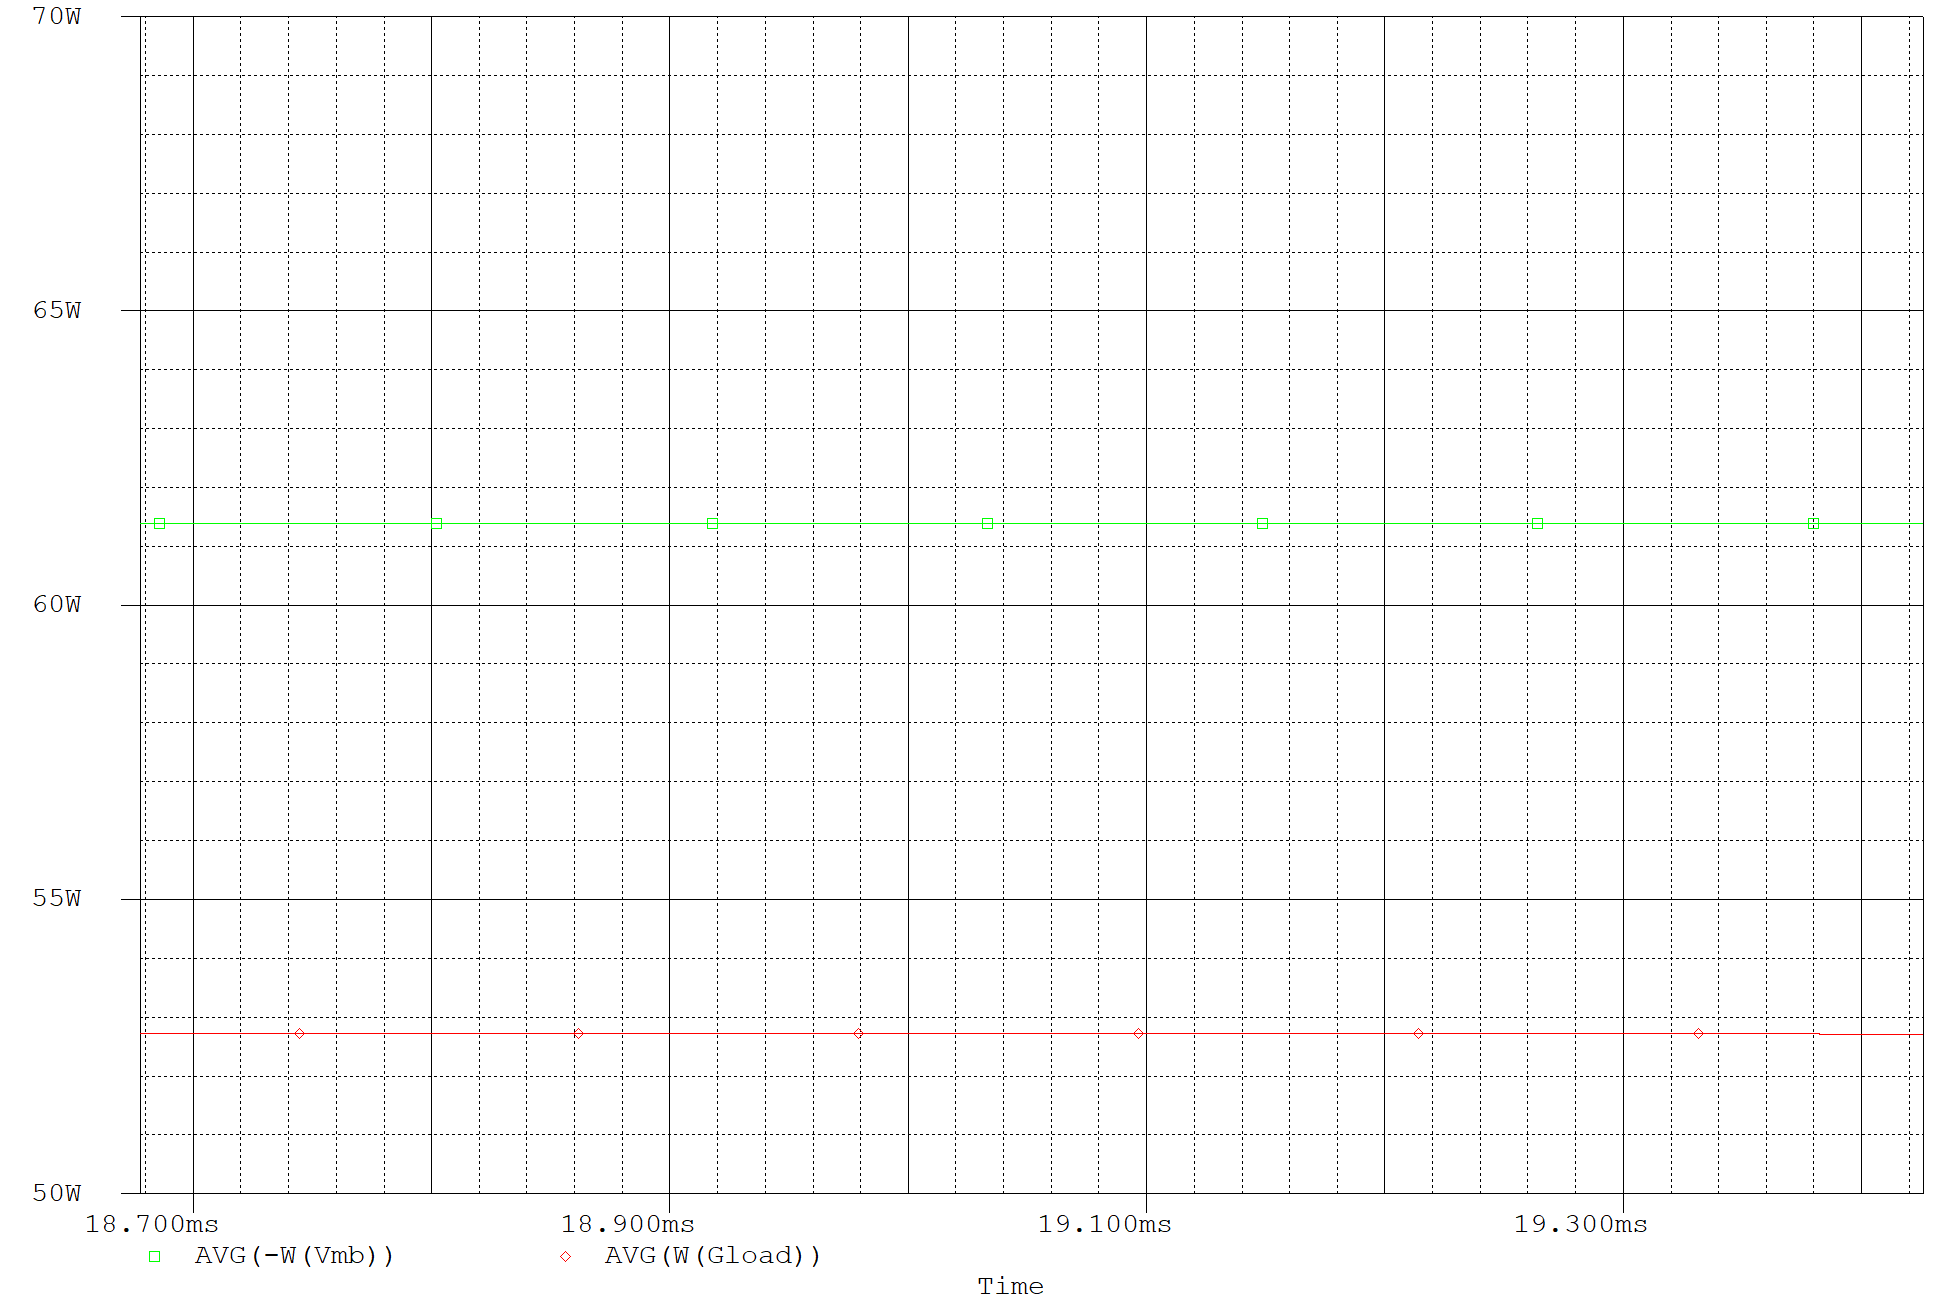
\includegraphics[max width=0.9\linewidth]{/tex/3iteration/billeder/Simulering/simulering_samlet_tab.png}
	\caption{Simulering af indgang- og udgangseffekt}
	\label{fig:simulering_power_samlet}
\end{figure}